\documentclass[12pt,a4paper]{article}
\usepackage[utf8]{inputenc}
\usepackage[spanish]{babel}
\usepackage[left=2.5cm,right=2.5cm,top=2cm,bottom=3.5cm]{geometry}
\usepackage{float}
\usepackage{graphicx} 
\usepackage{enumitem}
\usepackage{booktabs}
\usepackage{amsmath}
\usepackage[hidelinks]{hyperref}
\usepackage{parskip}
\setlength{\parindent}{1.27cm} 

\begin{document}

\begin{titlepage}
	\centering
	
\includegraphics[width=0.4\textwidth]{../../resources/logos/Nuevo-logo-UTB-1.png}\par\vspace{1.5cm} 
	{\scshape\LARGE\textbf{Universidad Tecnológica de Bolívar} \par}
	\vspace{1.5cm}
    \rule{\linewidth}{0.2 mm} \\[0.4 cm]
	{\huge\bfseries Análisis automatizado de caída libre mediante visión computacional y ajuste numérico \par} 
    \rule{\linewidth}{0.2 mm} \\[1.0 cm]
	\vspace{0.5cm}
	
	{\large\textbf{Actividad 2 - Primer corte} \par}
	\vspace{1.5cm}

    \centering{\emph{\textbf{Estudiantes:}}\\
        German De Armas Castaño \\ 
        Angel Vega Rodriguez \\
        Michael Taboada Naranjo\\}
        
    \vspace{1 cm}
    \centering{\emph{\textbf{Profesor:}}\\
        David Sierra Porta\\}
    
	\vfill
	{\large \today\par}
\end{titlepage}

\tableofcontents
\newpage

\section{Introducción}
Este reporte describe la metodología experimental y el análisis numérico del aplicativo diseñado para modelar la caída libre. A diferencia de los métodos rudimentarios que usan cronómetros manuales, este proyecto automatiza la extracción de datos utilizando avanzadas técnicas de visión por computadora.

Este enfoque evalúa y procesa los fotogramas de video para obtener la posición en función del tiempo, basándose en el modelo clásico de aceleración constante:
$$
y(t)=y_0+v_0 t+\frac{1}{2}gt^2,
$$
donde la aceleración de la gravedad $g$, la velocidad inicial $v_0$ y la posición inicial $y_0$ se calculan simultáneamente como parámetros variables del modelo.

\subsection{Planteamiento del problema}
La medición empírica de parámetros como la gravedad suele verse afectada negativamente por el error humano. El tiempo de reacción manual al usar un cronómetro es irregular e introduce sesgos muy grandes dentro de datos que se miden en simples fracciones de segundo, generando resultados que muchas veces carecen de sentido físico.

Para solucionar este obstáculo, el sistema propuesto elimina toda intervención humana en la medición utilizando una cámara de video con una tasa de fotogramas por segundo (FPS) constante. Si cada fotograma registra la posición $y$ del objeto en ese instante, el reloj se puede abstraer a gran precisión calculando el tiempo como $t = \frac{\text{frame}}{\text{FPS}}$. De esta manera, el error desproporcionado que introduce una persona se sustituye únicamente por el mínimo margen de desvío del sensor de la cámara, logrando mayor rigurosidad analítica.

\section{Técnicas Utilizadas y Metodología Computacional}
El sistema utiliza varios flujos de trabajo científicos importantes de Python: \texttt{OpenCV} para extraer fotogramas y detectar visualmente el objeto, \texttt{NumPy} para procesar los datos matemáticos numéricos, y \texttt{SciPy} para ajustar la curva final y minimizar el margen de error. El proceso base es el siguiente:

\subsection{Transformación Espacial (Calibración Dimensional)}
Las dimensiones que captura la cámara están definidas en una matriz finita medida en píxeles ($px$), pero toda evaluación física real necesita interpretarse en metros ($m$). Para resolver la conversión, se le solicita al usuario hacer clic sobre los extremos visuales de un objeto estático de tamaño conocido en la escena (como una regla métrica). Esto establece el factor físico de escala base:
$$
\text{Factor de escala} = \frac{\Delta px_{\text{regla}}}{\text{Longitud Real}_{\text{regla}}} \quad [\text{px/m}]
$$
\subsection{Procesamiento de la Imagen y Extracción de Puntos}
Para detectar una pelota real en caída, primero hay que lograr distinguirla sobre todos los colores que conforman el fondo. Para lograrlo, la imagen inicial captada (en formato estándar BGR) se transforma digitalmente al espacio de color y modelo cilíndrico HSV (Matiz, Saturación, Brillo):

\begin{enumerate}
    \item \textbf{Reducción de Escala (\textit{Downscaling}):} Para procesar el archivo más rápido, el sistema reduce la superficie de dimensiones del video a la mitad ($0.5\times$). Esta operación relaja la carga de rendimiento de la computadora notoriamente y en nada perjudica la precisión visual del cálculo de rastreo computacional.
    \item \textbf{Umbralización:} A través de la técnica \texttt{inRange}, el software aísla los espacios cromáticos y elabora una máscara temporal, la cual conserva de forma binaria a los píxeles que empaten con el color configurado por el usuario.
    \item \textbf{Morfología matemática:} Aplicando las operaciones filtro de \texttt{MORPH\_OPEN} y \texttt{MORPH\_CLOSE} sobre rejillas de $5\times 5$, se terminan de borrar imperfecciones microscópicas, como refracción de destellos o sombras secundarias esporádicas.
    \item \textbf{Cálculo del Centroide:} Ya obtenida la silueta en blanco limpia de la pelota detectada, se extraen sus estocásticos "Momentos de Imagen" espaciales ($M$). A través de un simple cruce, la computadora puede apuntar un punto exacto a sus coordenadas centrales ($(c_x, c_y)$) presentes a lo largo de este fotograma particular:
    $$ c_x = \frac{M_{10}}{M_{00}}, \quad\quad c_y = \frac{M_{01}}{M_{00}} $$
\end{enumerate}

\subsection{Ajuste del Modelo No Lineal Múltiple}
Una vez el video ha cerrado su recolección de base de datos emparejando coordenadas en formato metros en contraposición al tiempo deducido, el cálculo empuja estos vectores al optimizador algorítmico \texttt{curve\_fit} (cuya lógica responde al sistema no-lineal numérico de Levenberg-Marquardt).

A diferencia de un análisis manual tradicional que fuerza la constante original a valores absolutos (encontrar únicamente la $g$ pura o un intercepto sin sentido), este método automático permite que el programa ajuste con total libertad matemática tres parámetros clave ($y_0$, $v_0$ y $g$) buscando amoldar a la perfección el dictamen dictado de la ecuación real $ y(t) = y_0 + v_0 t + \frac{1}{2}gt^2$:

    \begin{itemize}
        \item El parámetro \textbf{\texttt{popt}} guarda las estimaciones concurrentes óptimas de caída libre ($y_0, v_0, g$). Constituye el vector resolutivo directo que satisface la mínima tolerancia de error sumado en los trazos de puntos registrados teórica y prácticamente:
        $$ \mathbf{popt} = \underset{y_0, v_0, g}{\text{arg min}} \sum_{i=1}^{N} \left( y_i - (y_0 + v_0t_i + \frac{g}{2}t_i^2) \right)^2 $$
        \item La matriz \textbf{\texttt{pcov}} representa la matriz final $3\times3$ de covarianza para las inferencias, la cual indica el confiable y respectivo margen en el que se ubicaría una aserción errónea o fallida de precisión sobre la probabilidad final del programa.
    \end{itemize}

\section{Arquitectura del Servidor Backend}
Dado que el procesamiento de lectura de imágenes es demasiado demandante para cualquier navegador web básico frontal, este se apoya integralmente y delega la ejecución al lenguaje base Python bajo la estructura \texttt{FastAPI}. Esta decisión de arquitectura subyacente separa e invoca las librerías poderosas en C (\texttt{OpenCV / NumPy}) mientras se comunica por rutinas REST asíncronas descritas a continuación.

\subsection{Ingesta, decodificación y mapeo paramétrico (\texttt{/upload} y \texttt{/preview})}
El ciclo de recabación de datos despierta cuando el experimentador direcciona y provee el material de evaluación enviándolo directamente desde el frontend a la ruta programada \texttt{/upload} vía una directiva \texttt{POST}. 

Al cargarse este video crudo estéticamente a la memoria veloz, el servidor invoca internamente sus motores \texttt{cv2.VideoCapture} logrando capturar detalles intrínsecos ocultos y elementales como la propia tasa original del archivo (\textit{Constante FPS}). Simultáneamente y de manera ingeniosa, extrae también su fotograma $t=0\text{s}$, lo transforma digitalmente en codificación \textbf{Base64 (JPEG)} y se lo reporta crípticamente a la vista frontal en respuesta. Esto alivia una carga de tráfico enorme, haciendo que la persona no tenga que volver a descargar todo el vídeo original, permitiéndole interactuar tranquilamente con la interfaz usando una imagen estática. Adicionalmente, rutas modulares ligeras operacionales GET, llamadas \texttt{/preview} y \texttt{/mask}, devuelven representaciones transitorias fotograma por fotograma para comprobar empíricamente que la configuración selectiva HSV concuerda perfectamente frente el cuerpo visible antes de darle pie al flujo mayor de análisis analítico final.

\subsection{Procesamiento Analítico Asíncrono (\texttt{/analyze\_stream})}
Si el sistema se tomara el trabajo rígido de computar linealmente fotograma a fotograma un video denso sincrónicamente, el sitio web principal perdería su renderizado causando cierres por límite de latencias de protocolo.

Superando tal asfixia colindante, la ejecución API instaura eficazmente un puente progresivo \textit{Server-Sent Events} (\textbf{SSE}), codificado con ráfagas NDJSON secuenciales. Bajo iteraciones ininterrumpidas continuas por debajo (\texttt{yield}), por cada frame real exitosamente depurado, el programa genera un pequeño aviso de evento asíncrono transmitido de vuelta por la red y renderizado gradualmente (ej. \texttt{\{"type": "progress", "y": 643, "t": 0.53\}}). Logrando que, en la vista macro general, estas actualizaciones de texto puntuales se consoliden dibujando proactivamente un seguimiento paralelo.

\subsection{Detección Autónoma del Suceso Cinemático (Derivadas Numéricas)}
Analizar un vídeo general involucra afrontar el gran abismo inicial cuando la persona vacila dudosa sosteniendo estáticamente por largos milisegundos la masa esférica y los saltos erráticos consecutivos poschoques en la superficie terminal. Encomendar mecánicamente datos defectuosos y sucios arrastraría una desviación de falla en \texttt{curve\_fit} hacia estimaciones ilógicas sin propósito.

La ingeniería que implementa el script \texttt{engine.py} depura tales sesgos abordando aproximaciones puras de vectores que modelizan velocidades y varianzas parcializadas y colindantes. Se evalúan y se sacan cuentas aproximando derivadas numéricas contiguas de primer plano:
$$ \mathbf{\vec{V}}_i \approx \frac{ \Delta \mathbf{Y}_i }{ \Delta t_i } = \frac{\mathbf{Y}_i - \mathbf{Y}_{i-1}}{t_i - t_{i-1}} $$

Se recorta de la muestra estadística absoluta de manera analítica cualquier iteración donde la propulsión y velocidad neta haya recaído debajo de los $0.05 \text{ m/s}$ (o sin correlatividad confirmada por al menos 3 ciclos). Mediante este embudo subyugante, se aísla únicamente la cronometría activa real y libre (redifinendo esta brecha depurada analítica como $t=0$) introduciendo verdaderamente valores congruentes en un único frente dinámico que la herramienta estadística ajusta en toda serenidad.

\section{Flujo Práctico de Procesamiento del Aplicativo}
La lógica explicada anteriormente se estructura tras bambalinas bajo una interfaz web visual, sumamente fácil y fluida para que cualquier experimentador evalúe su estudio por caída libre desde 4 pasos de configuración simples documentados iterativamente:

\subsection{Carga de Video y Calibración Espacial}
El proceso práctico inicia cuando se arrastra la muestra de archivo empírico hacia la web y se pausa el lienzo base indexado $t=0$ para interactividad inicial (véase la Figura \ref{fig:calibracion}).

Al investigador principal se le encarga de dar dos clics superficiales concretos delimitando una estructura geométrica conocida dentro de la previsualización (\textit{e.g.} regla o listón emparejado con el fondo). El frente aplica el teorema Pitagórico $\Delta px = \sqrt{(x_2-x_1)^2 + (y_2 - y_1)^2}$ para desglosar la diferencia escalar de esta distancia métrica; pidiendo acto subsiguiente llenar manualmente cuánto midió esa regla real. Este paso provee sin rodeos algorítmicos la constante $\lambda = \frac{m}{\text{px}}$ posibilitando todo encuadre numérico matemático posterior que requiera mediciones y longitudes estandarizadas.

\begin{figure}[H]
    \centering
    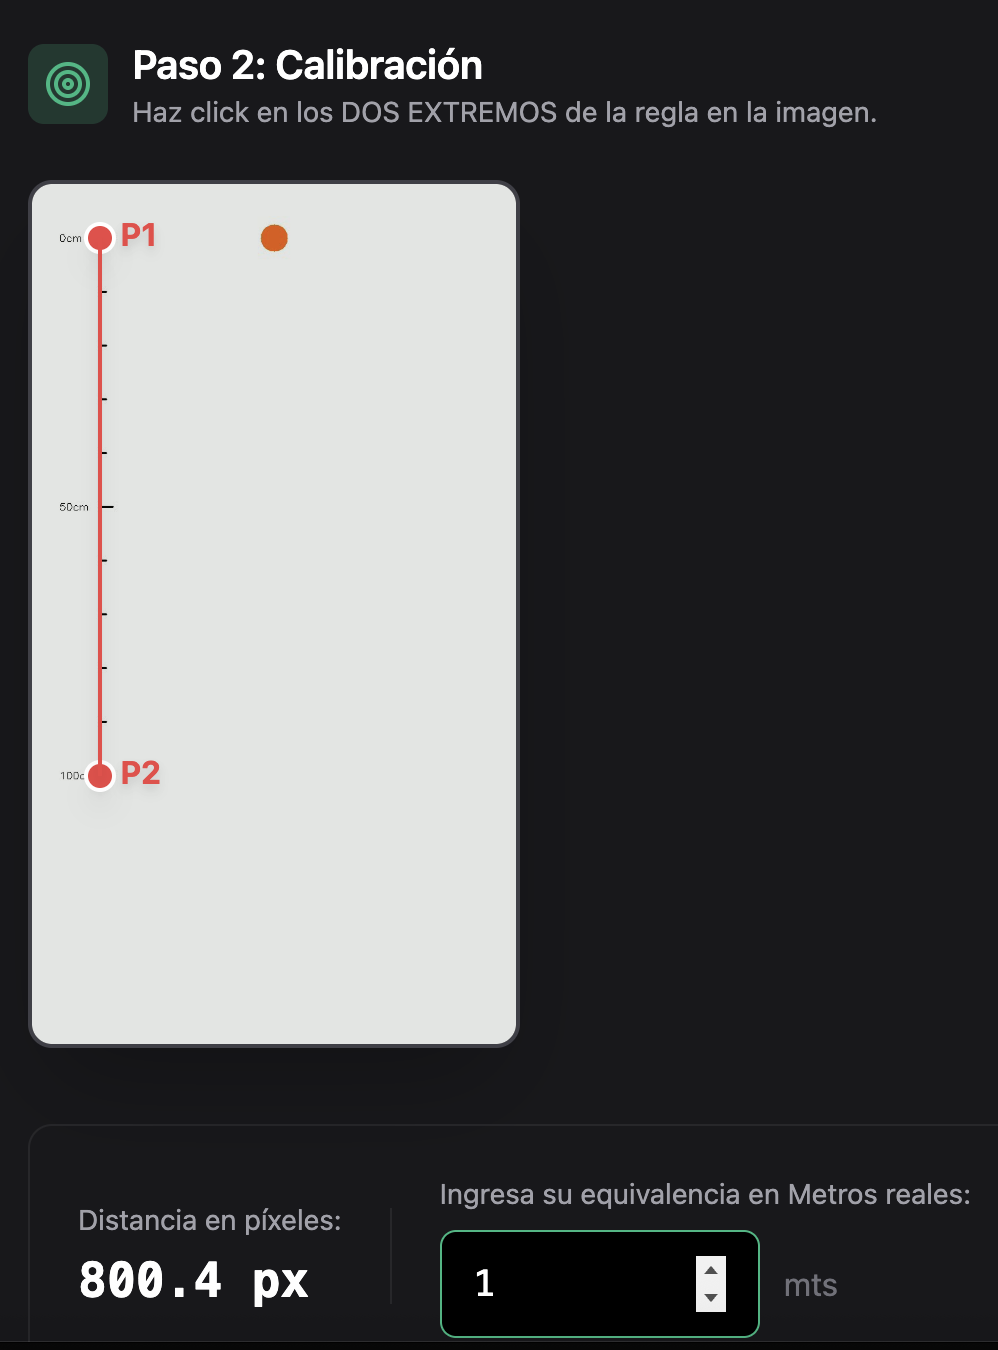
\includegraphics[width=0.35\linewidth]{imgs/calibracion.png}
    \caption{Lienzo de calibración definiendo el factor de escala sobre la referencia grabada.}
    \label{fig:calibracion}
\end{figure}

\subsection{Ajuste Paramétrico del Filtro Cromático (HSV)}
Concluido lo referente a distancia, la siguiente prioridad es apuntalear las cualidades focales de un color en solitario frente a sus luces. Utilizando entonces seis bandas cilíndricas independientes de control deslizante en propiedades HSV, al ser accionadas individualmente reaccionan dinámicamente destruyendo \texttt{cv2.inRange} la iluminación remanente externa, resguardando netamente perfiles lumínicos encasillados y delimitados sobre la estructura central particular para que sea una mancha oscura y depurada (conforme exhibe interactivamente la Figura \ref{fig:mascara_hsv}).

\begin{figure}[H]
    \centering
    \begin{minipage}{0.48\textwidth}
        \centering
        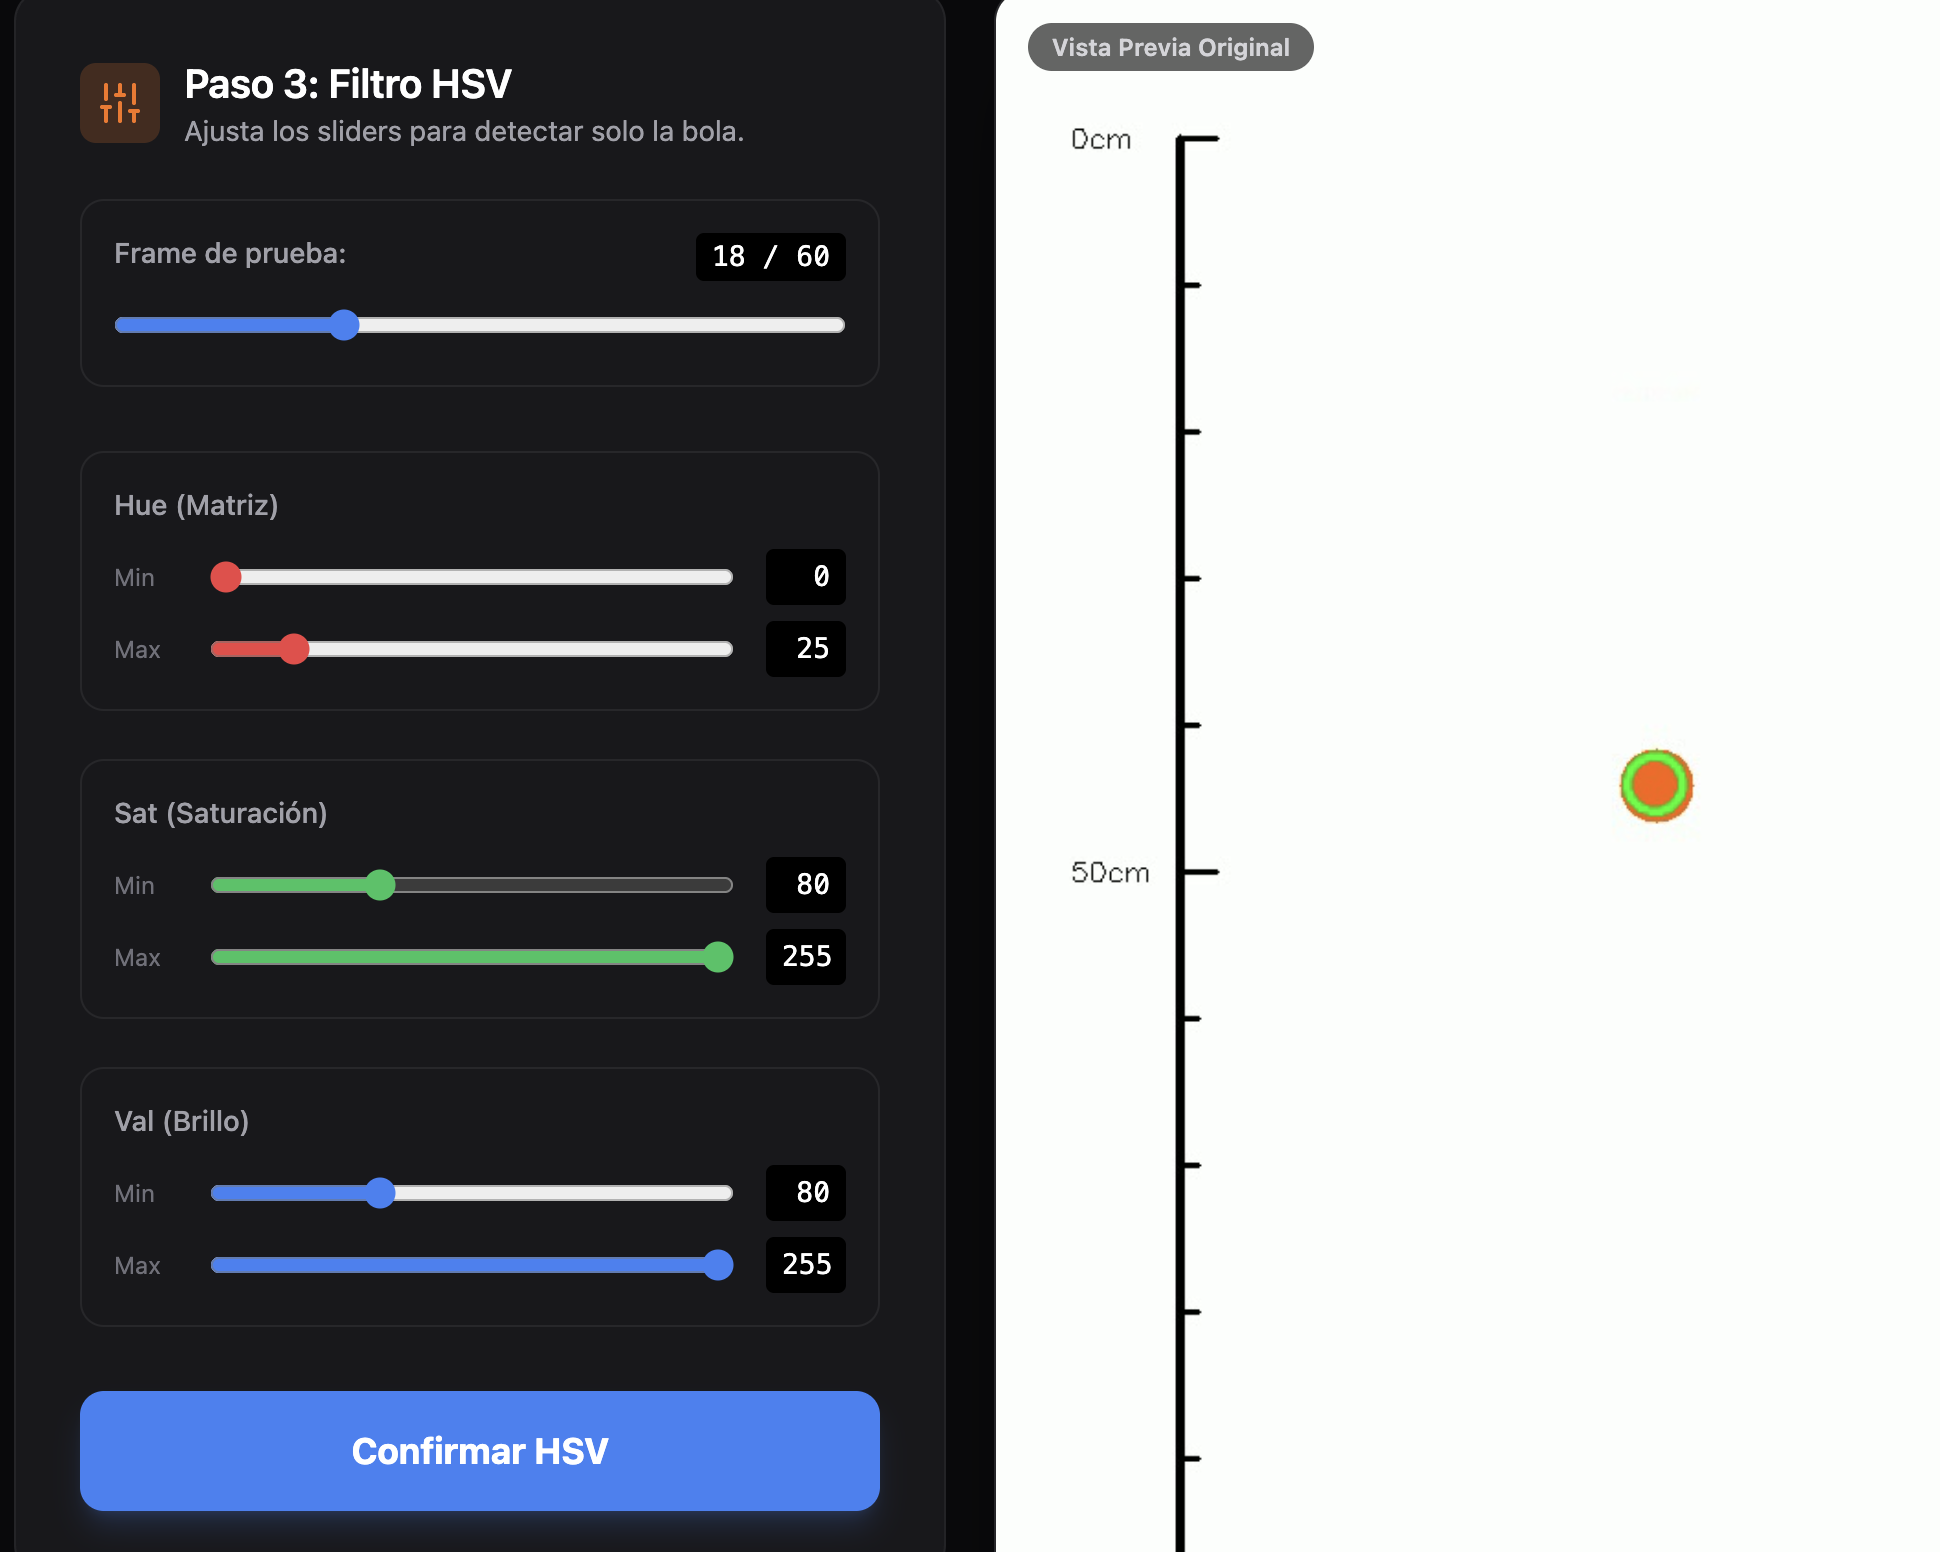
\includegraphics[width=0.85\linewidth]{imgs/filtro-hsv.png}
        \caption{Identificación del rastro con el filtro paramétrico HSV.}
        \label{fig:filtro_hsv}
    \end{minipage}\hfill
    \begin{minipage}{0.48\textwidth}
        \centering
        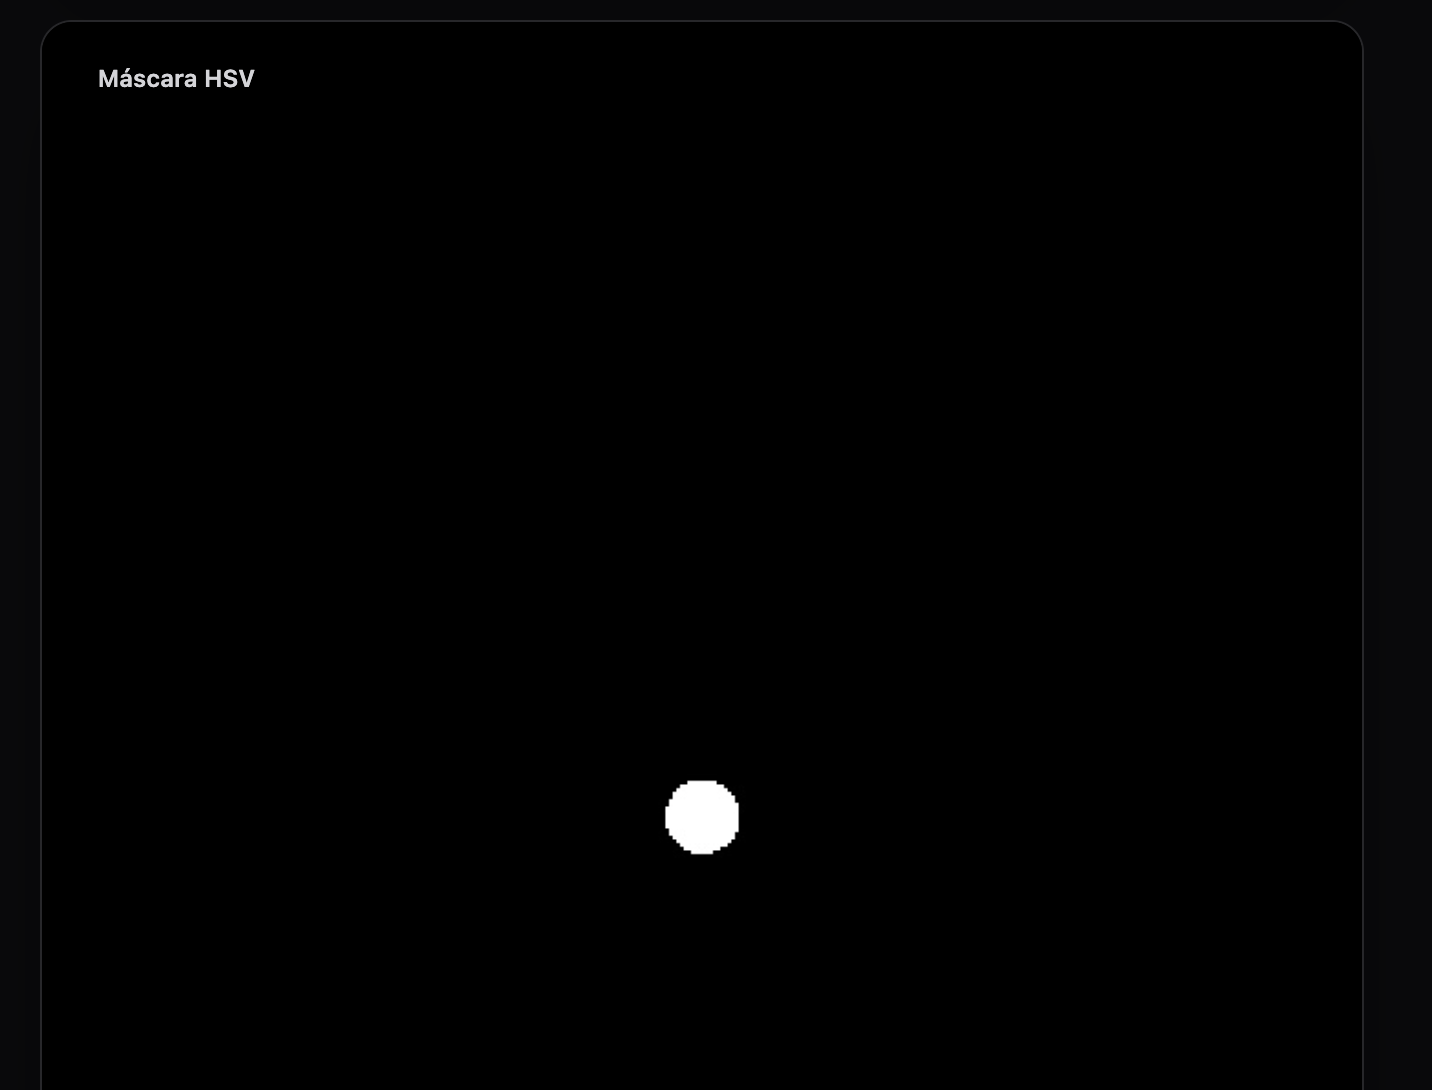
\includegraphics[width=0.85\linewidth]{imgs/mascara-hsv.png}
        \caption{Refracción binarizada abstracta resultante (Máscara).}
        \label{fig:mascara_hsv}
    \end{minipage}
\end{figure}

\subsection{Detección Continua (Tracking de Fotogramas)}
Subyugados el ajuste general para filtrar un vector contorno con matiz apropiado, el experimentador puede invocar el disparo en tiempo real ejecutando "Analizar Video". Ocultando de forma desatendida sus mecanismos internos, todo el metraje es pasado por los filtros revisando cada par de iteraciones sus propiedades numéricas perimetrales $M_{10}$ y $M_{00}$. Dejándole visualizar al operador empírico final, en su propia terminal interactiva web, trazos de rastreos anillados dibujándose simultáneamente fotograma a fotograma como garantía paralela explícita de recolección ininterrumpida de resultados del motor (tal como ilustra cabalmente la Figura \ref{fig:detecciones}).

\begin{figure}[H]
    \centering
    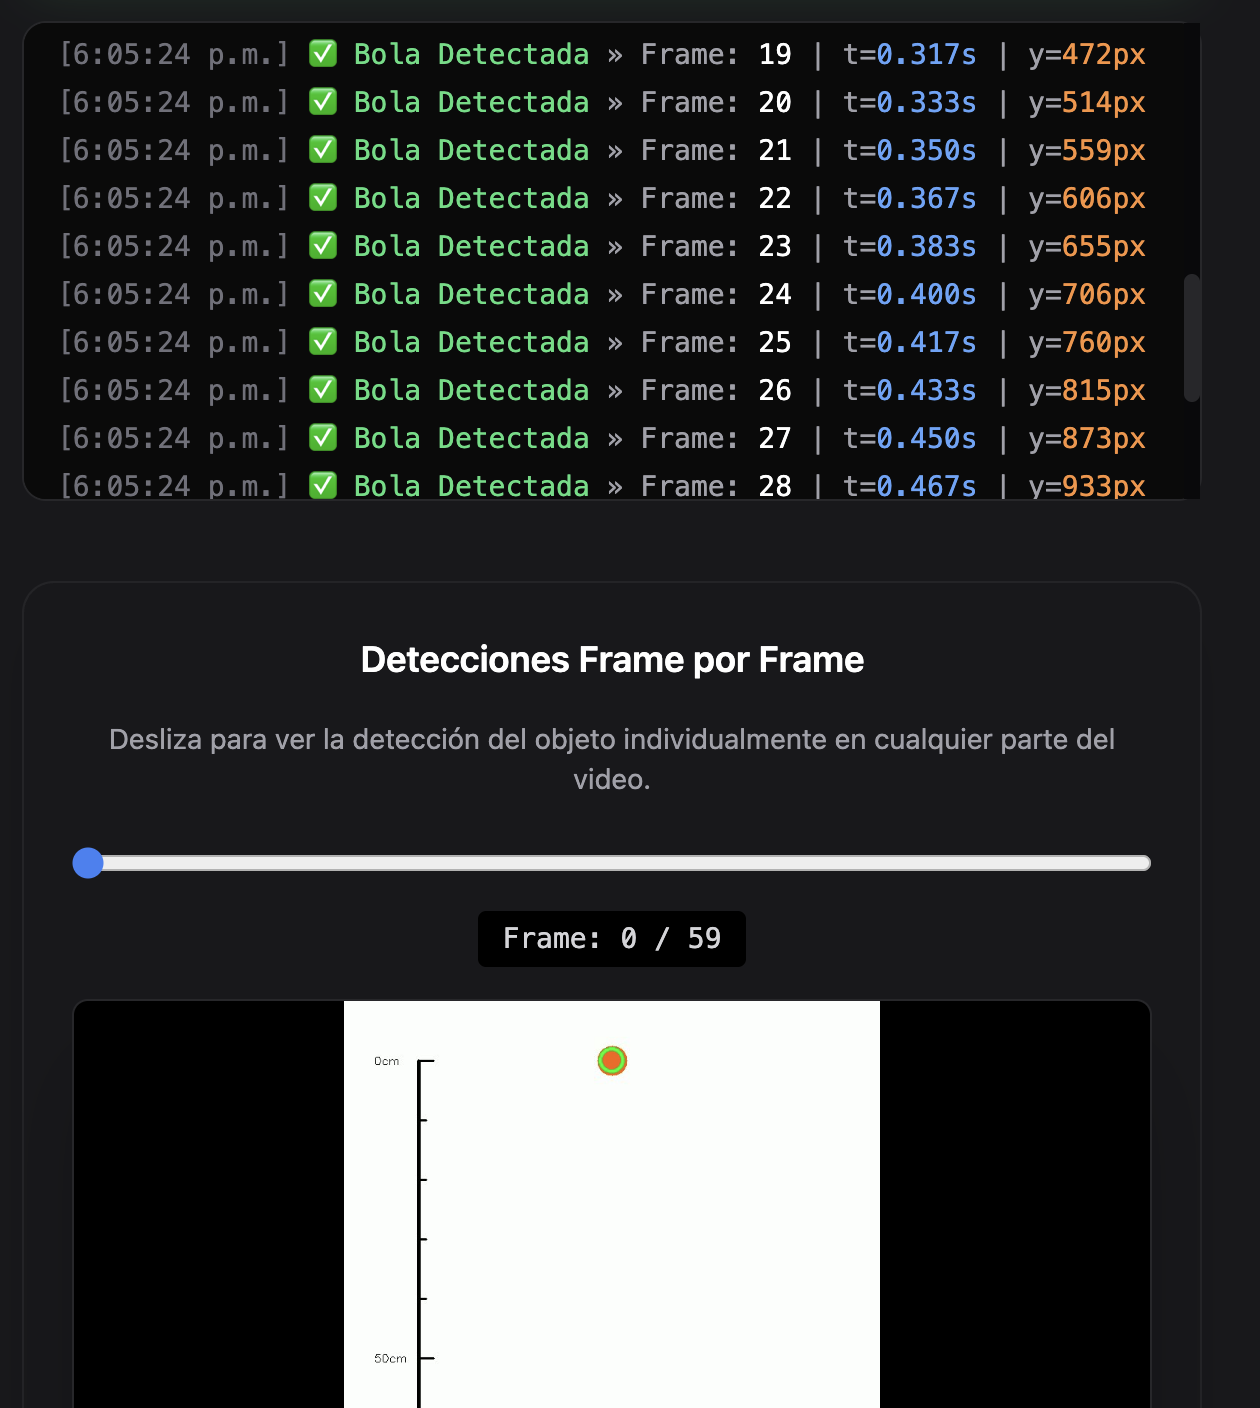
\includegraphics[width=0.55\linewidth]{imgs/deteccion-frames.png}
    \caption{Barrido de la señal capturando la pelota cuadro a cuadro progresivamente.}
    \label{fig:detecciones}
\end{figure}

\subsection{Extracción de Resultados Matemáticos}
En el instante donde termina la ingesta visual vectorial y las derivadas concluyen en delimitar asertivamente el rango unipolar positivo acelerado, el sistema consolida los márgenes de gradiente unificados presentándolos al panel derecho visual bajo \textit{SciPy} (véase la Figura \ref{fig:resultados_panel}). Esta sección consolida las sumatorias visualizando el esparcimiento estadístico experimental ajustándose férreamente en la figura parabólica clásica, extrayendo parámetros de Gravedad $g$ de resoluciones incontestables frente a los estándares de cronometría erráticos experimentales comunes.

\begin{figure}[H]
    \centering
    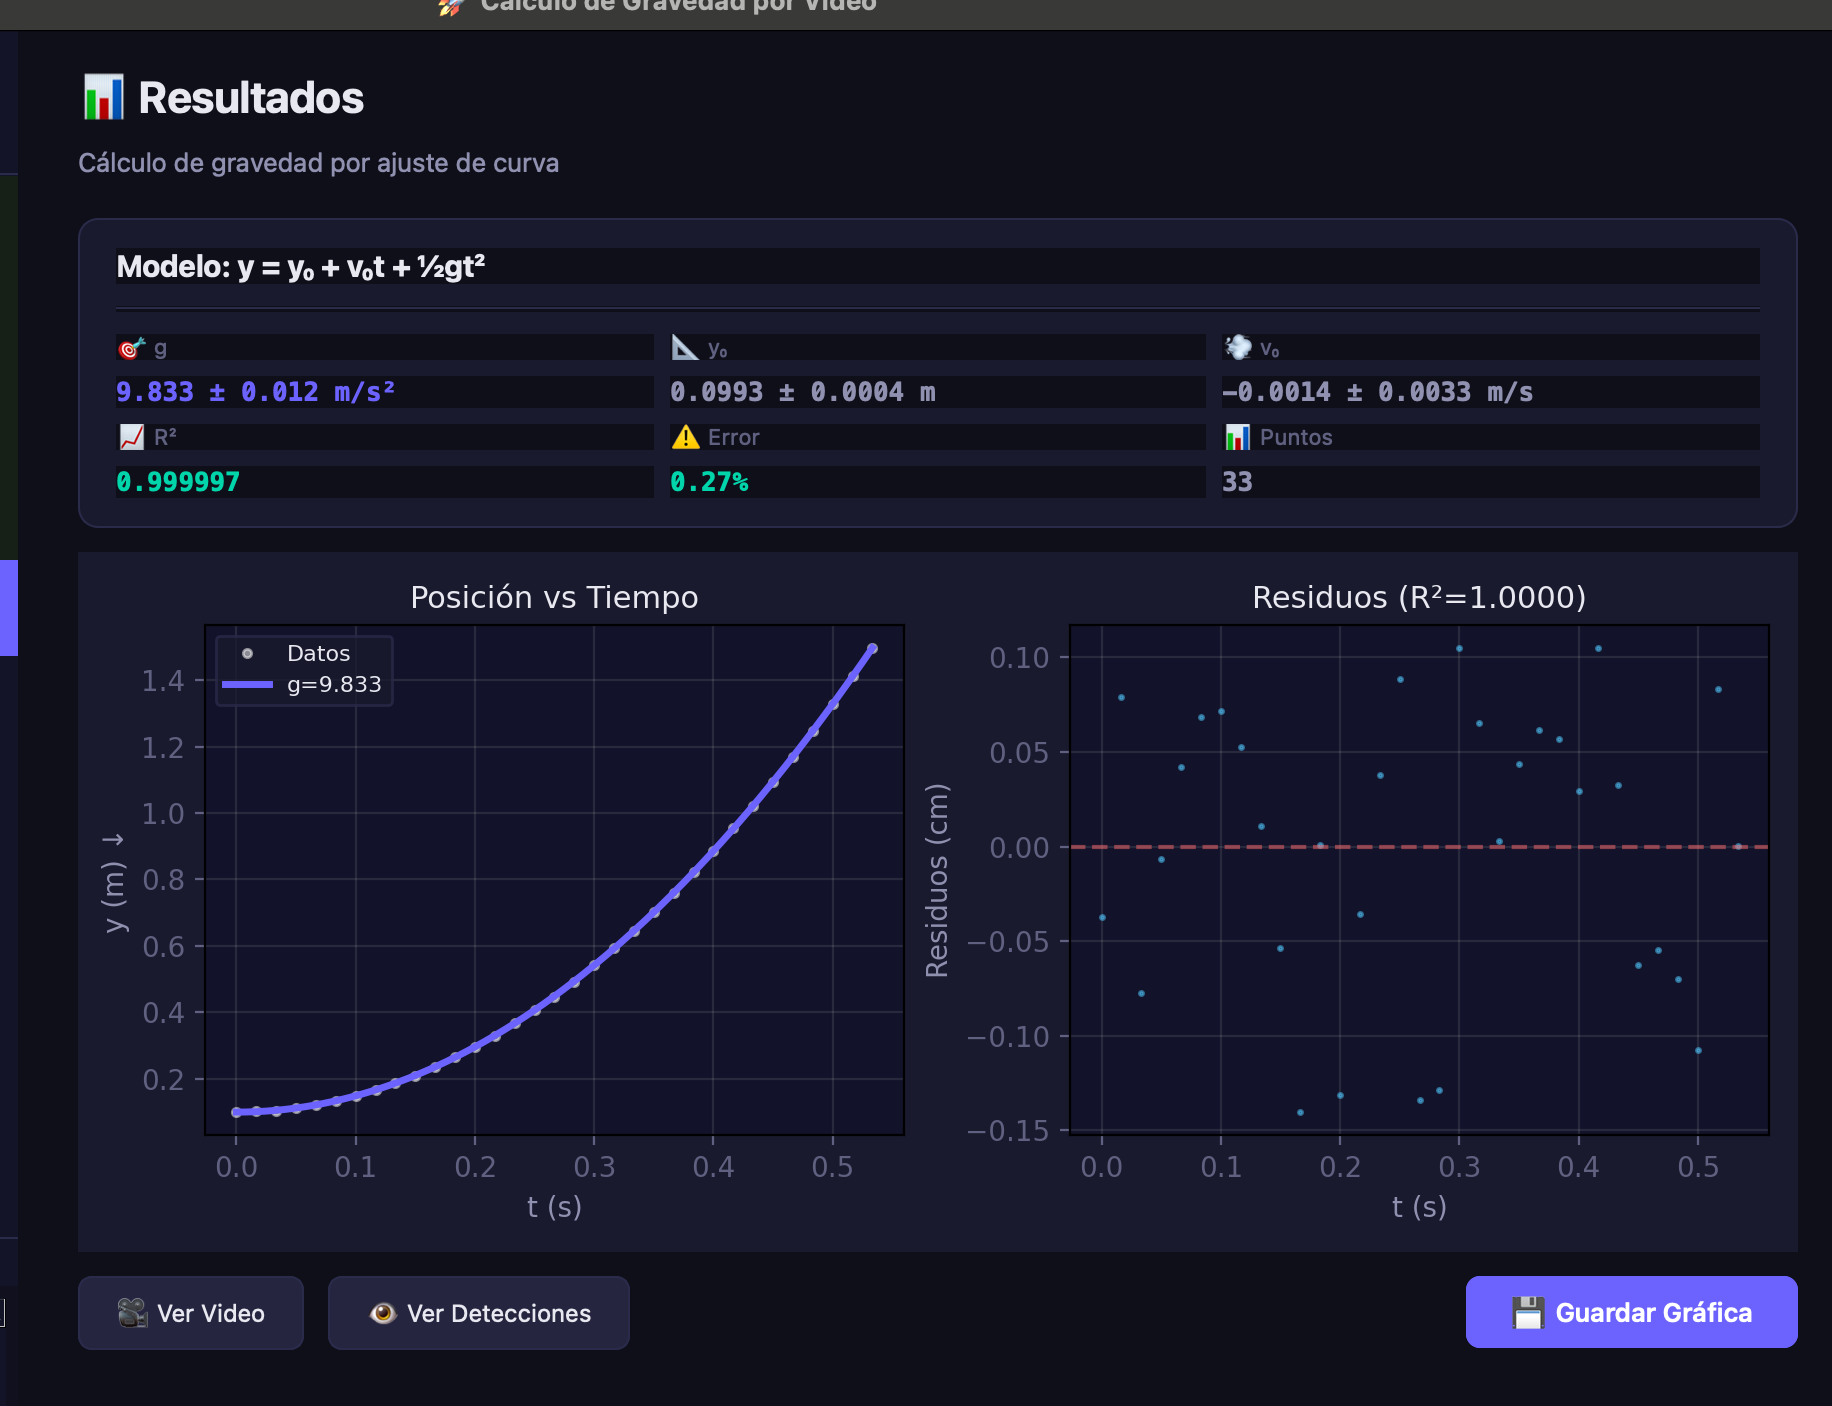
\includegraphics[width=0.75\linewidth]{imgs/resultados.png}
    \caption{Consola interactiva de resultados consolidando el parámetro final de Gravedad y bondad de ajuste.}
    \label{fig:resultados_panel}
\end{figure}

\section{Resultados y Análisis Comparativo de Errores}
Gracias a que este sistema excluye con rigor automatizado casi en toda dimensión la latencia e imperfección humana manual, los valores teóricos se acercan y aproximan estrechamente a modelos ideales universales de cálculo numérico en un porcentaje analítico superior de residual $R^2 \approx 0.99$.

Del mismo modo, admitir que estas matrices evalúen un encuadre real tridimensional sobre la recolección, dota a la base predictiva de absorber imperfecciones marginales de desajuste originario como el factor $v_0$. Demostrando así contundentemente que la liberación real física por el ser humano añade un arrastre asimétrico no lineal, evidenciando un realismo paramétrico subyacente impensable del lado matemático rústico tradicional sin optimización de iteración actual que era forzado artificialmente a arrancar sin fricciones en ceros precisos estadísticos.

\section{Conclusiones}
La restructuración tecnológica integral asíncrona por parte este software analítico interactivo con lógicas OpenCV exigen y muestran verdaderamente las deficiencias estadísticas de recolecciones con métodos ordinarios mecánicos. Analizar ininterrumpidamente frecuencias regulares matriciales en bases computacionales borra gran sesgo sistematizado perjudicial convirtiendo toda falla de rastreo final como incidentes ínfimos de tipo fotográfico aleatorio con márgenes fácilmente anulables con las sumatorias asintóticas que evalúa el motor matemático de regresiones `SciPy curve\_fit`.

Este macroproyecto valida lógicamente a gran escala que los métodos programáticos para solucionar o rastrear fenómenos de cinemática Newtoniana reales superan inquebrantablemente a cualquier inferencia base pre-establecida y ratifica el gran avance aplicativo práctico en aislar puramente fenómenos mecánicos eliminando todo sesgo disonante con variables no-lineales subyugadas a rigor analítico estandarizado.

\newpage
\begin{thebibliography}{9}

\bibitem{resnick} 
Halliday, D., Resnick, R. y Krane, K. S. (2002).
\textit{Física (Vol. 1)}. Grupo Editorial Patria.

\bibitem{opencv_morph} 
OpenCV Documentation. (n.d.). 
\textit{Morphological Transformations}. Open Source Computer Vision Library. Recuperado de \url{https://docs.opencv.org/master/d9/d61/tutorial_py_morphological_ops.html}

\bibitem{opencv_moments} 
OpenCV Documentation. (n.d.). 
\textit{Contour Features - Image Moments}. Open Source Computer Vision Library. Recuperado de \url{https://docs.opencv.org/master/dd/d49/tutorial_py_contour_features.html}

\bibitem{scipy_curve_fit} 
SciPy.org. (n.d.). 
\textit{scipy.optimize.curve\_fit}. Documentación oficial de la librería SciPy v1.11.x. Recuperado de \url{https://docs.scipy.org/doc/scipy/reference/generated/scipy.optimize.curve_fit.html}

\bibitem{numpy_doc} 
NumPy API Reference. (n.d.). 
\textit{Mathematical functions and Array Manipulation}. Documentación Oficial NumPy. Recuperado de \url{https://numpy.org/doc/stable/reference/}

\bibitem{fastapi_sse} 
FastAPI framework. (n.d.). 
\textit{Custom Response - HTML, Stream, File, others - StreamingResponse}. Documentación oficial FastAPI. Recuperado de \url{https://fastapi.tiangolo.com/advanced/custom-response/}

\end{thebibliography}

\end{document}